\documentclass[11pt,a4paper]{article}
\usepackage[margin=1in]{geometry}
\usepackage{graphicx}
\usepackage{booktabs}
\usepackage{amsmath}
\usepackage{hyperref}
\usepackage{xcolor}
\usepackage{caption}
\usepackage{subcaption}
\usepackage{float}

\title{RankAlign Training Dynamics Analysis\\
\large When Does RankAlign / TC Improve?}
\author{Automated Analysis Report}
\date{June 9, 2026}

\begin{document}
\maketitle

\begin{abstract}
This report analyzes training dynamics for RankAlign models across four model/task combinations (gemma-2-9b-it and Qwen3.5-9B on membership and IFEval tasks). We characterize \textbf{(a)} when RankAlign improves correlation over the base model, \textbf{(b)} when the full method improves over basic RankAlign, and \textbf{(c)} when typicality correction (TC) specifically improves over non-TC training. We also report training diagnostics from WandB logs and additional statistics (concordance, score delta distributions).
\end{abstract}

\tableofcontents
\newpage

%% ============================================================
\section{Q1: When Does Each Component Help?}
%% ============================================================

\subsection{Main Comparison: Gen ROC AUC (TC, Self-Scoring)}

Table~\ref{tab:main_comparison} shows the generator ROC AUC (typicality-corrected) for the final model (epoch 2) evaluated on the training set with self-TC scoring.

\begin{table}[H]
\centering
\caption{Generator ROC AUC (TC, self-scoring) at epoch 2. Bold = best per row. $\Delta$ relative to base.}
\label{tab:main_comparison}
\begin{tabular}{lcccccc}
\toprule
\textbf{Model / Task} & \textbf{Base} & \textbf{s1 (SFT)} & \textbf{s2 (RA basic)} & \textbf{s4 (RA full)} & \textbf{s3 (TC-self)} \\
\midrule
Gemma / Membership & 0.851 & --- & 0.941 & 0.948 & \textbf{0.976} \\
Gemma / IFEval    & 0.670 & 0.586 & 0.482 & 0.753 & \textbf{0.801} \\
Qwen / Membership  & 0.799 & 0.902 & 0.880 & 0.899 & \textbf{0.969} \\
Qwen / IFEval     & 0.606 & 0.599 & 0.558 & 0.711 & \textbf{0.743} \\
\bottomrule
\end{tabular}
\end{table}

\subsection{Key Findings}

\begin{enumerate}
\item \textbf{s3 (TC-self) is the best setting in every single combination.}
\item \textbf{Basic RankAlign (s2) hurts on IFEval} --- Gemma IFEval drops from 0.670 to 0.482 (below chance). Without NLL constraints, generator scores explode.
\item \textbf{The full method (s4) consistently helps}, adding +0.08--0.11 over base across all combos.
\item \textbf{TC-self (s3) adds +0.03--0.07 over s4} --- a consistent, meaningful improvement from typicality-aware training.
\end{enumerate}

\subsection{Visualizations}

\begin{figure}[H]
\centering
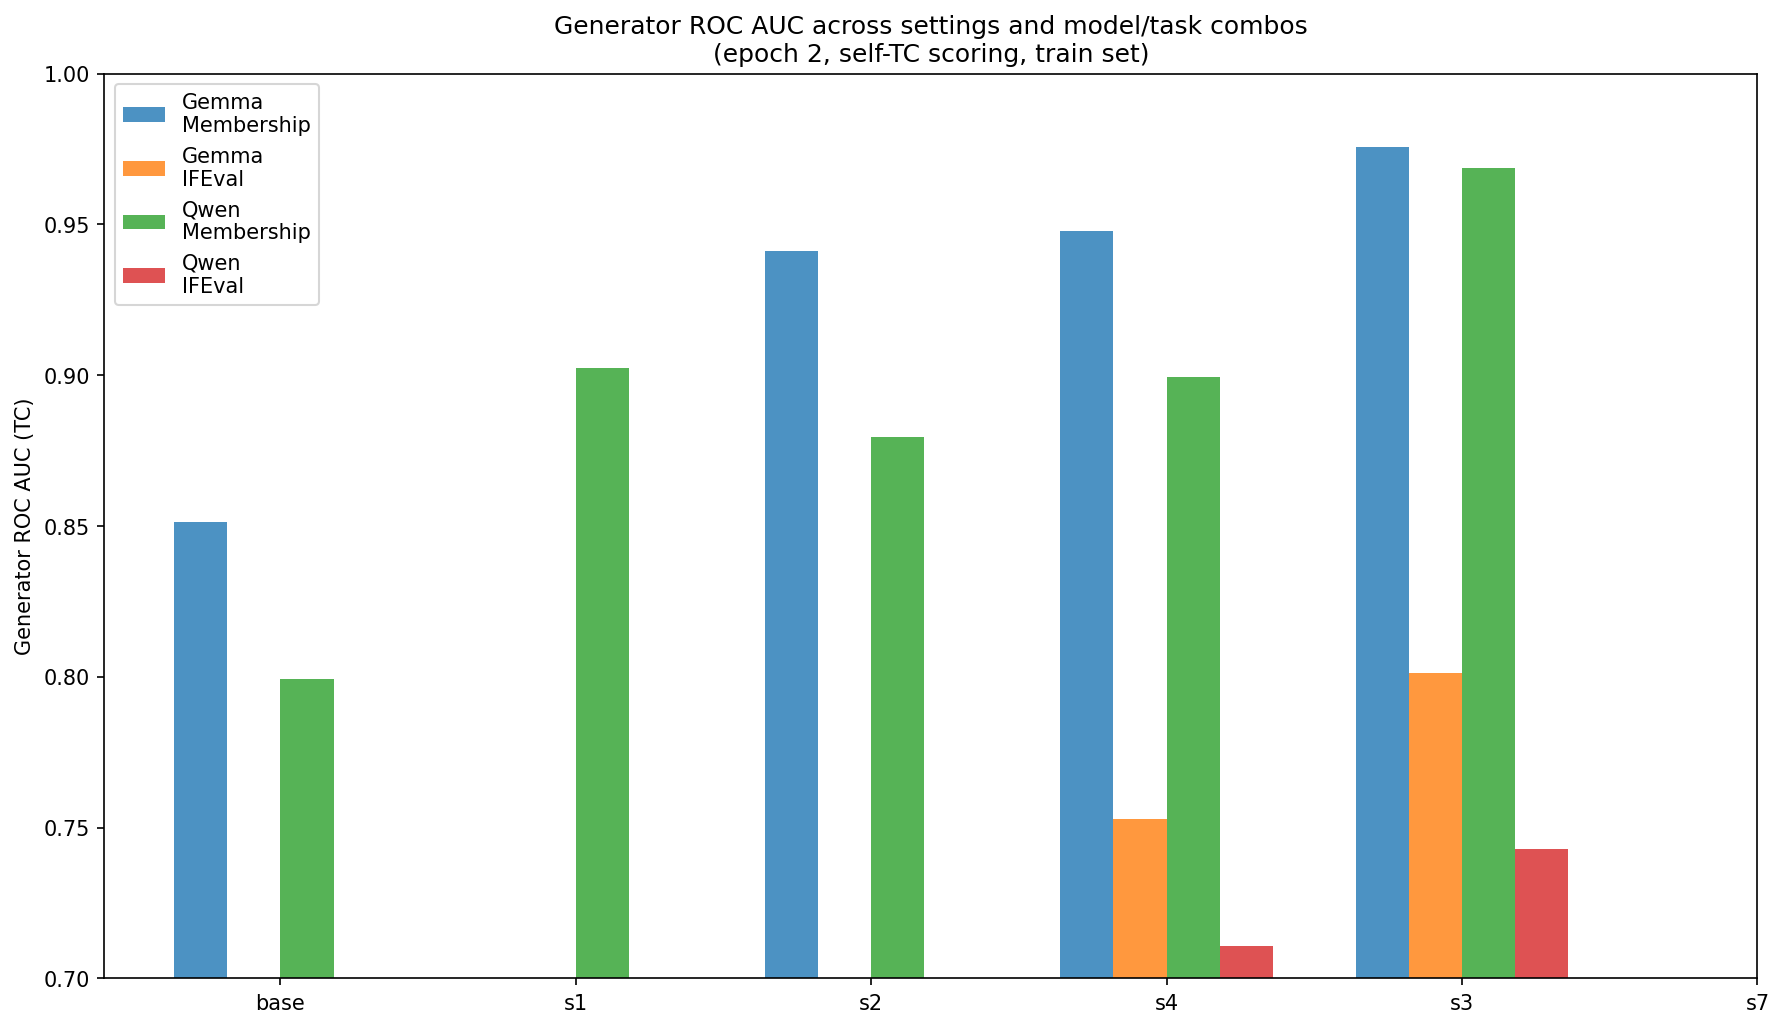
\includegraphics[width=0.95\textwidth]{plots/unified_genroc_comparison.png}
\caption{Generator ROC AUC across settings and model/task combinations (epoch 2, self-TC scoring, train set).}
\label{fig:unified_genroc}
\end{figure}

\begin{figure}[H]
\centering
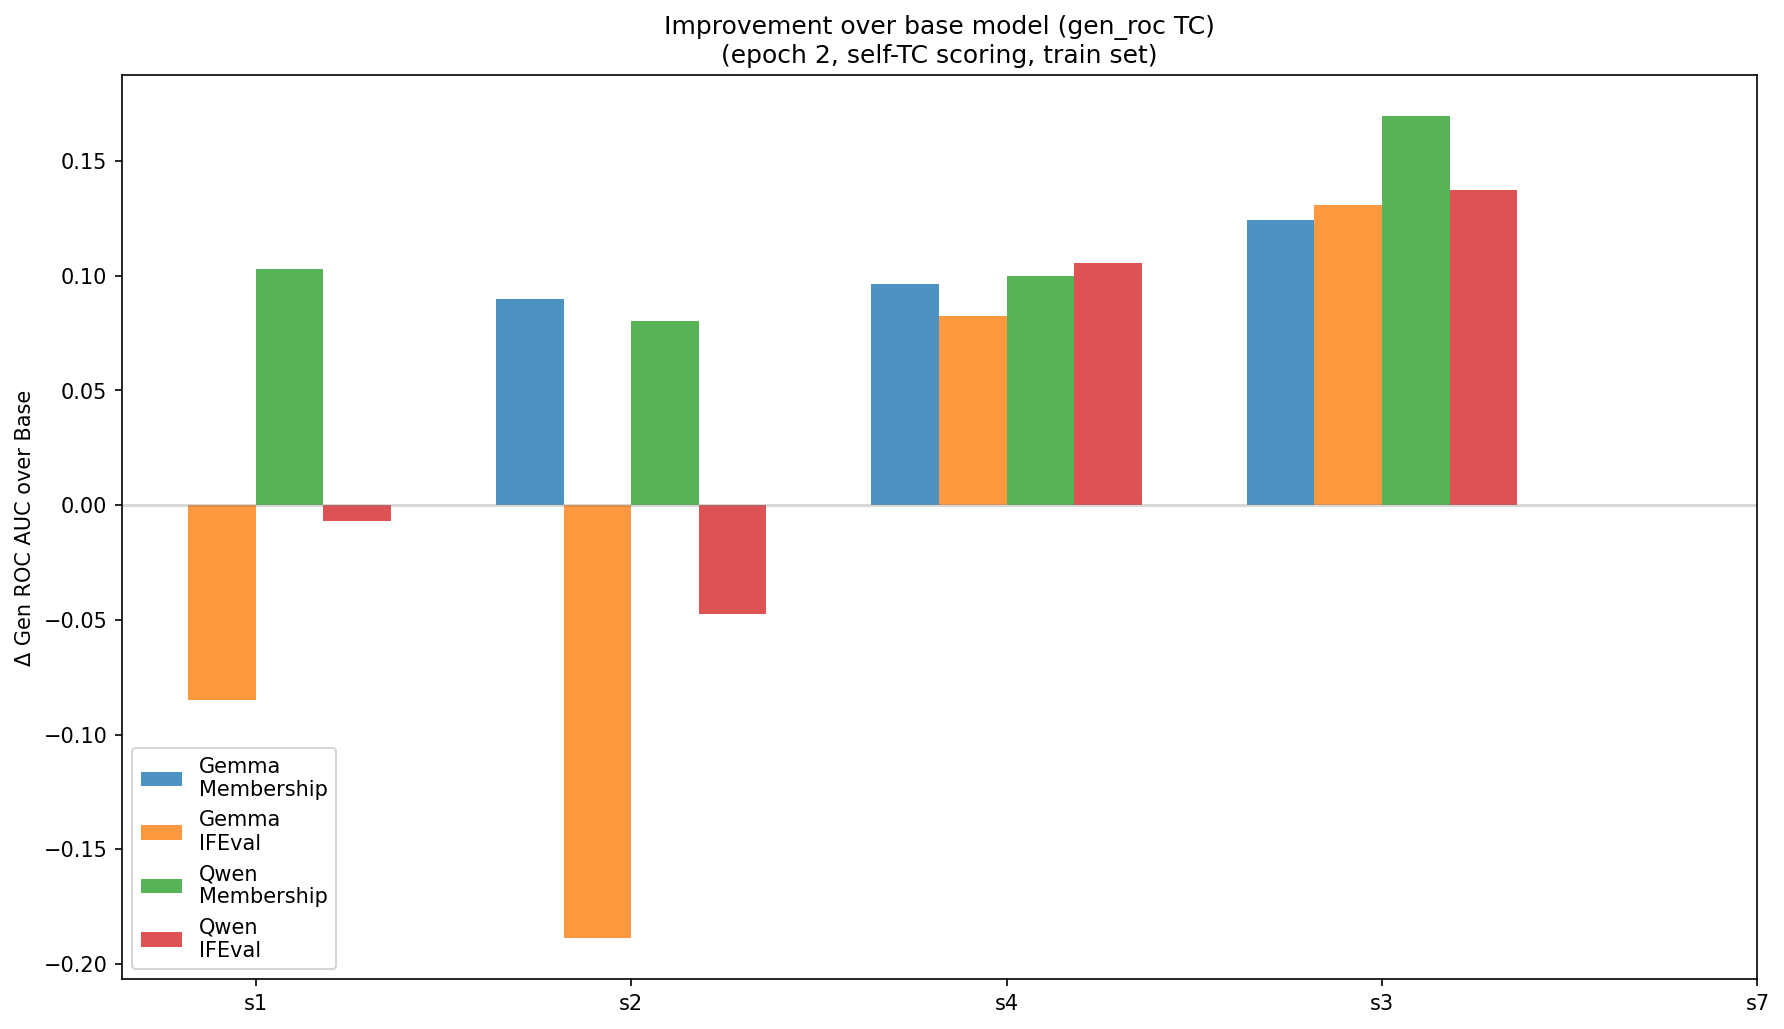
\includegraphics[width=0.95\textwidth]{plots/unified_improvement_over_base.png}
\caption{Improvement ($\Delta$) in gen ROC AUC over base model.}
\label{fig:improvement}
\end{figure}

%% ============================================================
\section{Q2: Training Diagnostics}
%% ============================================================

\subsection{Loss Curves from WandB}

Training was monitored via WandB for gemma-ifeval and qwen-membership/ifeval (gemma-membership was trained pre-WandB).

\begin{figure}[H]
\centering
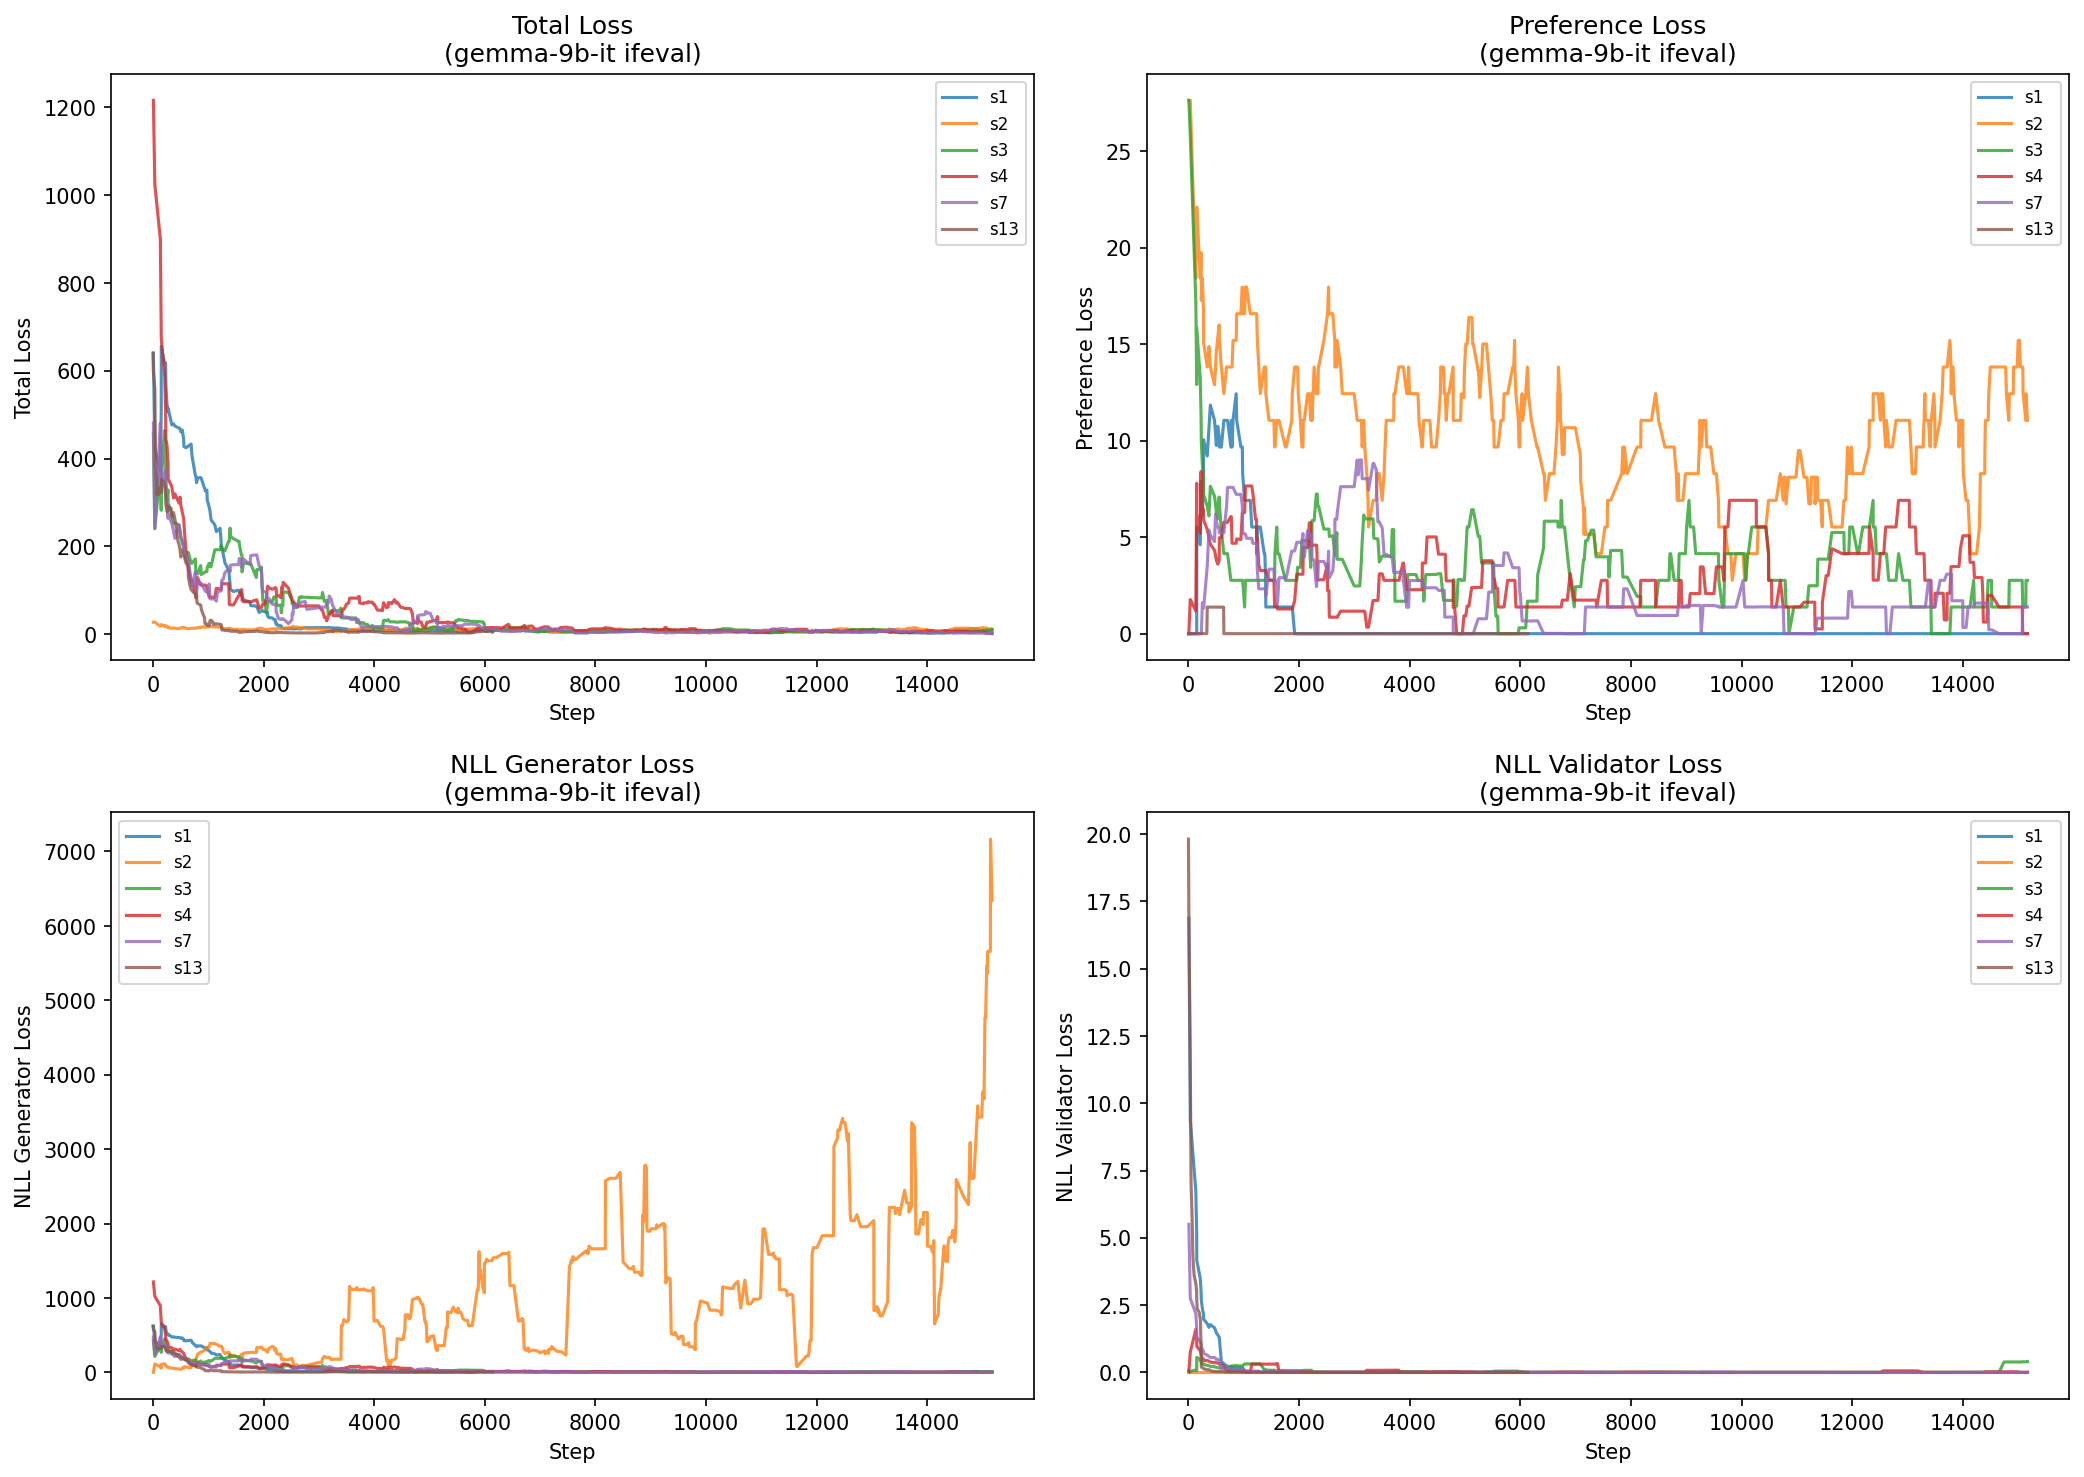
\includegraphics[width=0.95\textwidth]{plots/wandb_loss_curves_gemma-9b-it_ifeval.png}
\caption{Training loss curves for gemma-2-9b-it on IFEval.}
\label{fig:loss_gemma_ifeval}
\end{figure}

\begin{figure}[H]
\centering

\includegraphics[width=0.95\textwidth]{{plots/wandb_loss_curves_qwen3.5-9b_membership}.png}
\caption{Training loss curves for Qwen3.5-9B on membership.}
\label{fig:loss_qwen_mem}
\end{figure}

\begin{figure}[H]
\centering

\includegraphics[width=0.95\textwidth]{{plots/wandb_loss_curves_qwen3.5-9b_ifeval}.png}
\caption{Training loss curves for Qwen3.5-9B on IFEval.}
\label{fig:loss_qwen_ifeval}
\end{figure}

\subsection{Diagnostic Flags}

\begin{itemize}
\item \textbf{All settings}: High variance in the final training quarter. This is inherent to the ranking loss (pairs are noisy).
\item \textbf{s3 (gemma ifeval)}: NLL-V increases during training --- the validator signal degrades slightly as ranking dominates.
\item \textbf{s2, s4 (qwen ifeval)}: Total loss drifts upward --- correlates with s2's poor downstream metrics.
\end{itemize}

\subsection{Score Explosion Diagnostic}

A key diagnostic is the mean pairwise absolute difference in generator scores (gen\_delta\_mean). Large values indicate score explosion during training.

\begin{table}[H]
\centering
\caption{Generator score spread diagnostic. Values $>$1000 indicate training instability.}
\label{tab:score_explosion}
\begin{tabular}{llrrl}
\toprule
\textbf{Task} & \textbf{Setting} & \textbf{gen\_delta\_mean} & \textbf{gen\_roc} & \textbf{Status} \\
\midrule
Gemma IFEval & s2 (basic) & 13,421 & 0.482 & \textcolor{red}{Exploded} \\
Gemma IFEval & s4 (full) & 691 & 0.753 & OK \\
Gemma IFEval & s3 (TC-self) & 216 & 0.801 & Best \\
\midrule
Qwen IFEval & s2 (basic) & 1,031 & 0.558 & \textcolor{orange}{Borderline} \\
Qwen IFEval & s4 (full) & 408 & 0.711 & OK \\
Qwen IFEval & s3 (TC-self) & 139 & 0.743 & Best \\
\midrule
Gemma Membership & s2 & 9.1 & 0.941 & OK \\
Gemma Membership & s4 & 10.9 & 0.948 & OK \\
Gemma Membership & s3 & 10.7 & 0.976 & Best \\
\bottomrule
\end{tabular}
\end{table}

\textbf{Pattern}: TC-self training produces the most compact score distributions (lowest gen\_delta\_mean) \emph{and} the best gen\_roc. The NLL constraints prevent explosion, and TC further tightens the score distribution.

%% ============================================================
\section{Q3: Additional Statistics}
%% ============================================================

\subsection{Generator-Validator Concordance}

Concordance measures the fraction of item pairs where the generator and validator agree on the ordering direction.

\begin{table}[H]
\centering
\caption{Concordance at epoch 2 (self-TC scoring). Chance = 0.5.}
\label{tab:concordance}
\begin{tabular}{lccccc}
\toprule
\textbf{Model / Task} & \textbf{Base} & \textbf{s1} & \textbf{s2} & \textbf{s4} & \textbf{s3} \\
\midrule
Gemma / Membership & 0.705 & --- & 0.794 & 0.787 & \textbf{0.803} \\
Gemma / IFEval & 0.548 & 0.561 & 0.370 & 0.677 & \textbf{0.694} \\
Qwen / Membership & 0.671 & 0.734 & 0.759 & 0.752 & \textbf{0.807} \\
Qwen / IFEval & 0.545 & 0.553 & 0.571 & 0.641 & \textbf{0.646} \\
\bottomrule
\end{tabular}
\end{table}

Note: s2 on Gemma IFEval has concordance 0.370 (below chance), confirming the generator scores are \emph{anti-correlated} with the validator.

\subsection{Spearman Correlation (Generator vs Validator)}

\begin{table}[H]
\centering
\caption{Spearman $\rho$ between generator and validator scores (epoch 2, self-TC).}
\label{tab:spearman}
\begin{tabular}{lccccc}
\toprule
\textbf{Model / Task} & \textbf{Base} & \textbf{s1} & \textbf{s2} & \textbf{s4} & \textbf{s3} \\
\midrule
Gemma / Membership & 0.585 & --- & 0.798 & 0.795 & \textbf{0.826} \\
Gemma / IFEval & 0.141 & 0.178 & $-$0.374 & 0.504 & \textbf{0.567} \\
Qwen / Membership & 0.496 & 0.665 & 0.723 & 0.715 & \textbf{0.830} \\
Qwen / IFEval & 0.119 & 0.151 & 0.205 & 0.404 & \textbf{0.431} \\
\bottomrule
\end{tabular}
\end{table}

\subsection{Score Delta Distributions}

\begin{figure}[H]
\centering
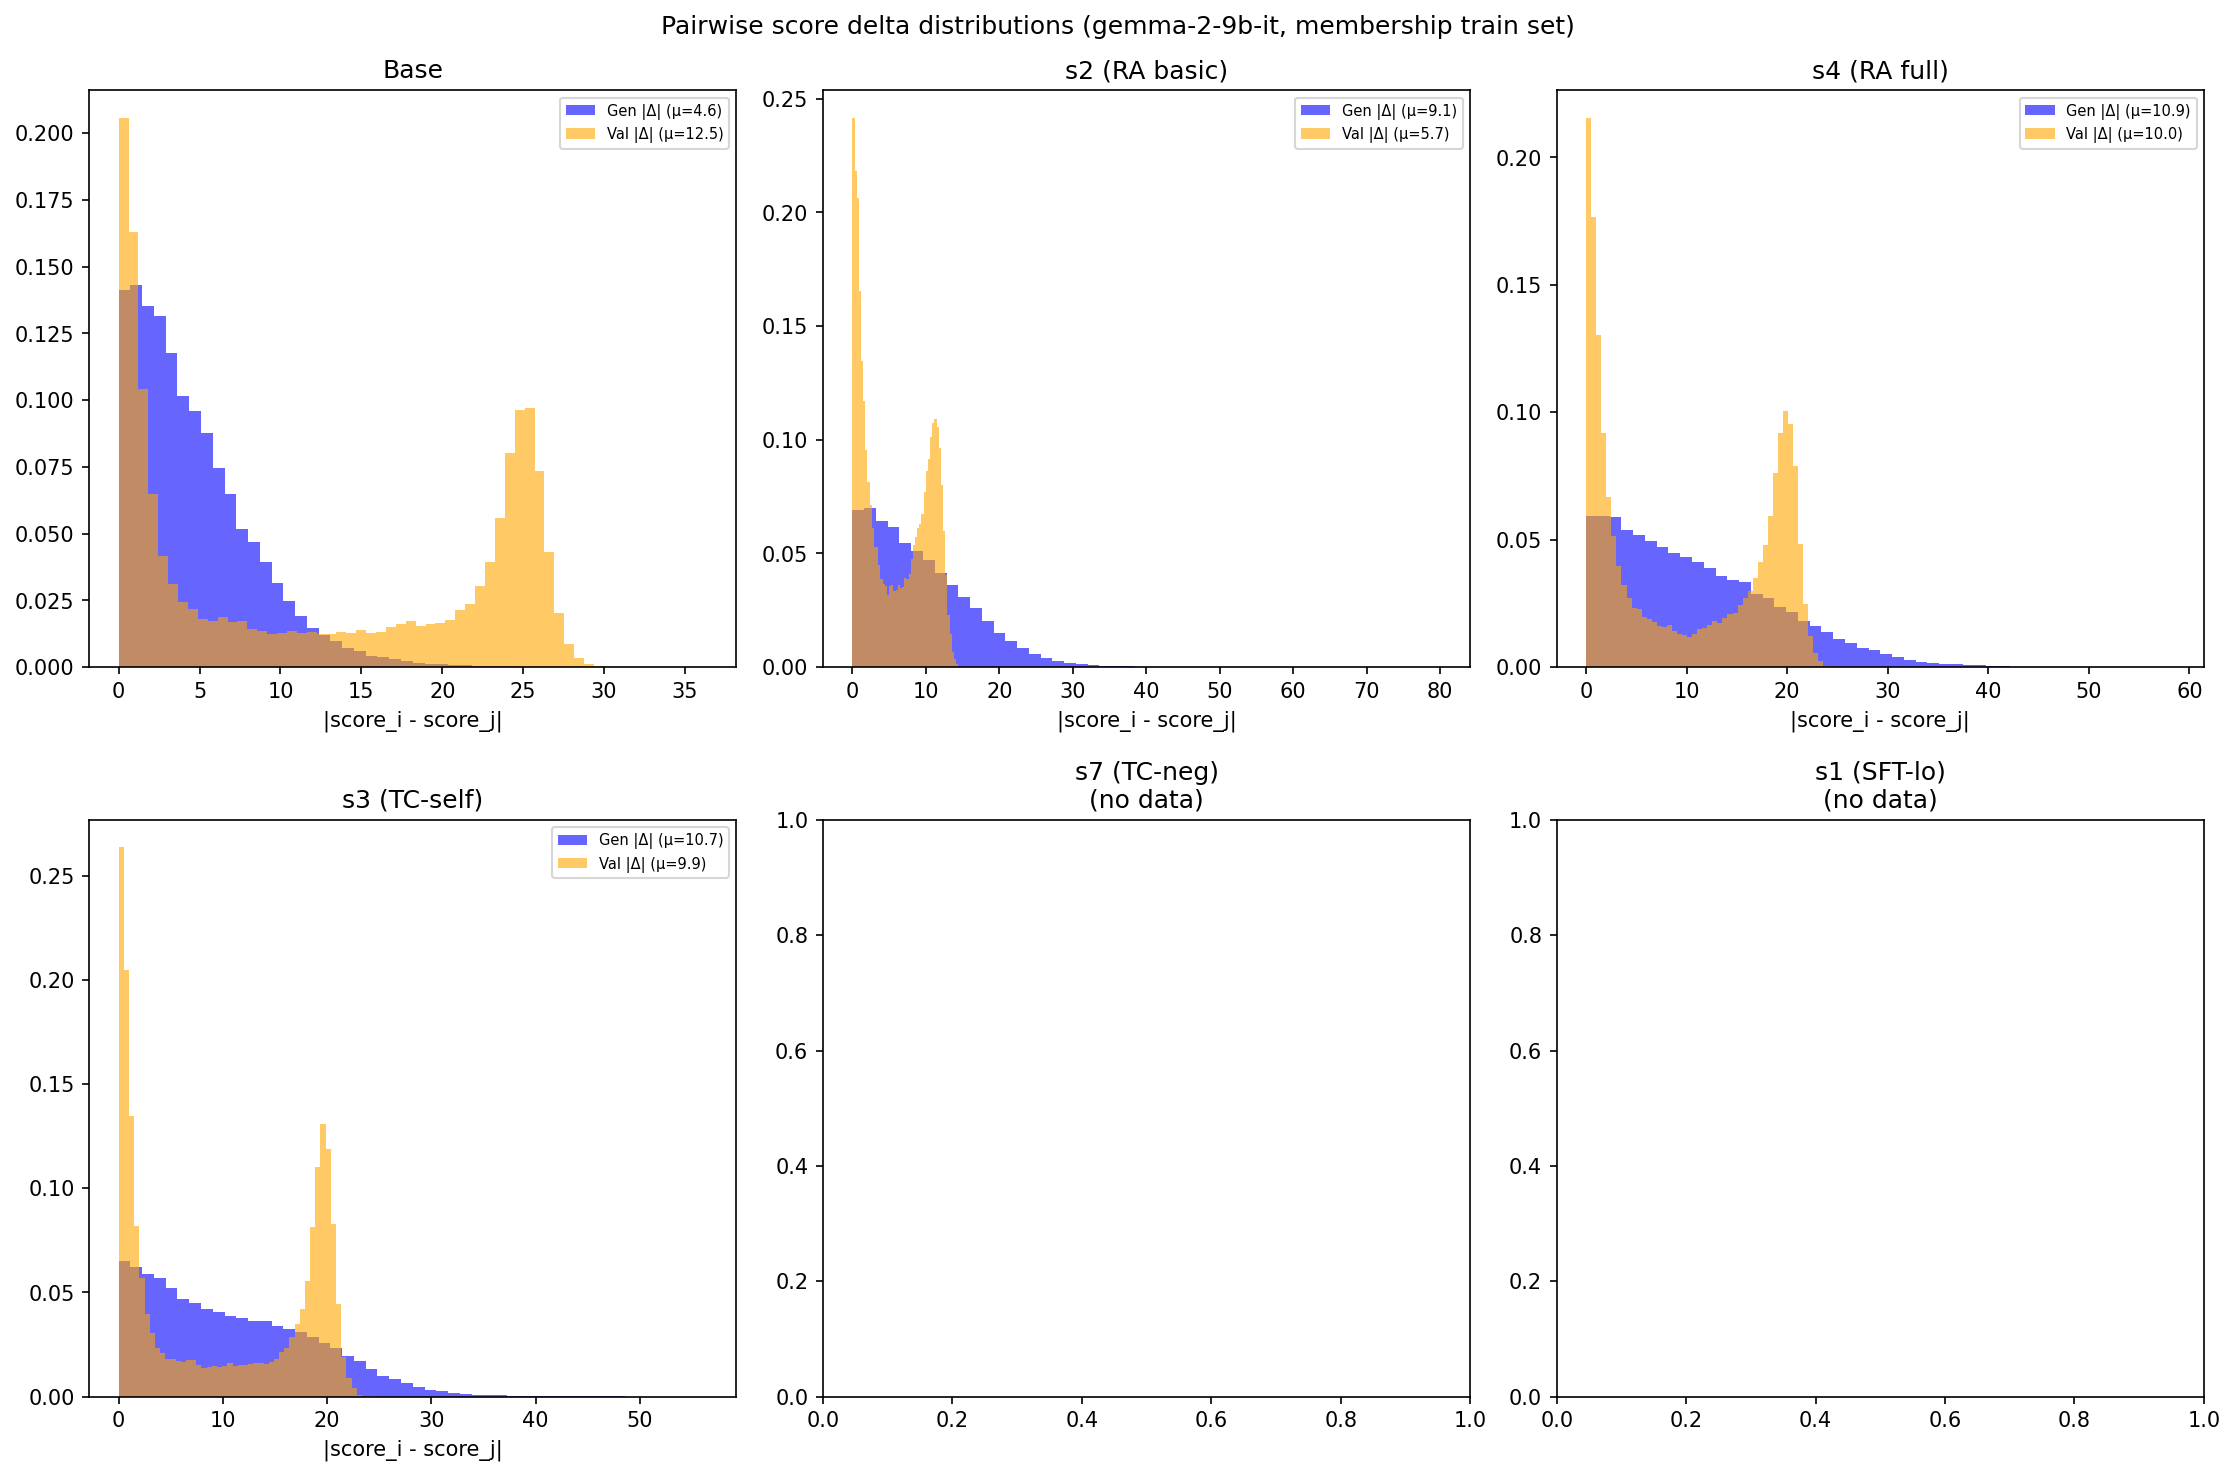
\includegraphics[width=0.95\textwidth]{plots/gemma_membership_delta_histograms.png}
\caption{Pairwise score delta distributions for gemma membership. Generator (blue) and validator (orange) distributions. Tighter = better calibrated.}
\label{fig:delta_histograms}
\end{figure}

\subsection{Training Dynamics}

\begin{figure}[H]
\centering
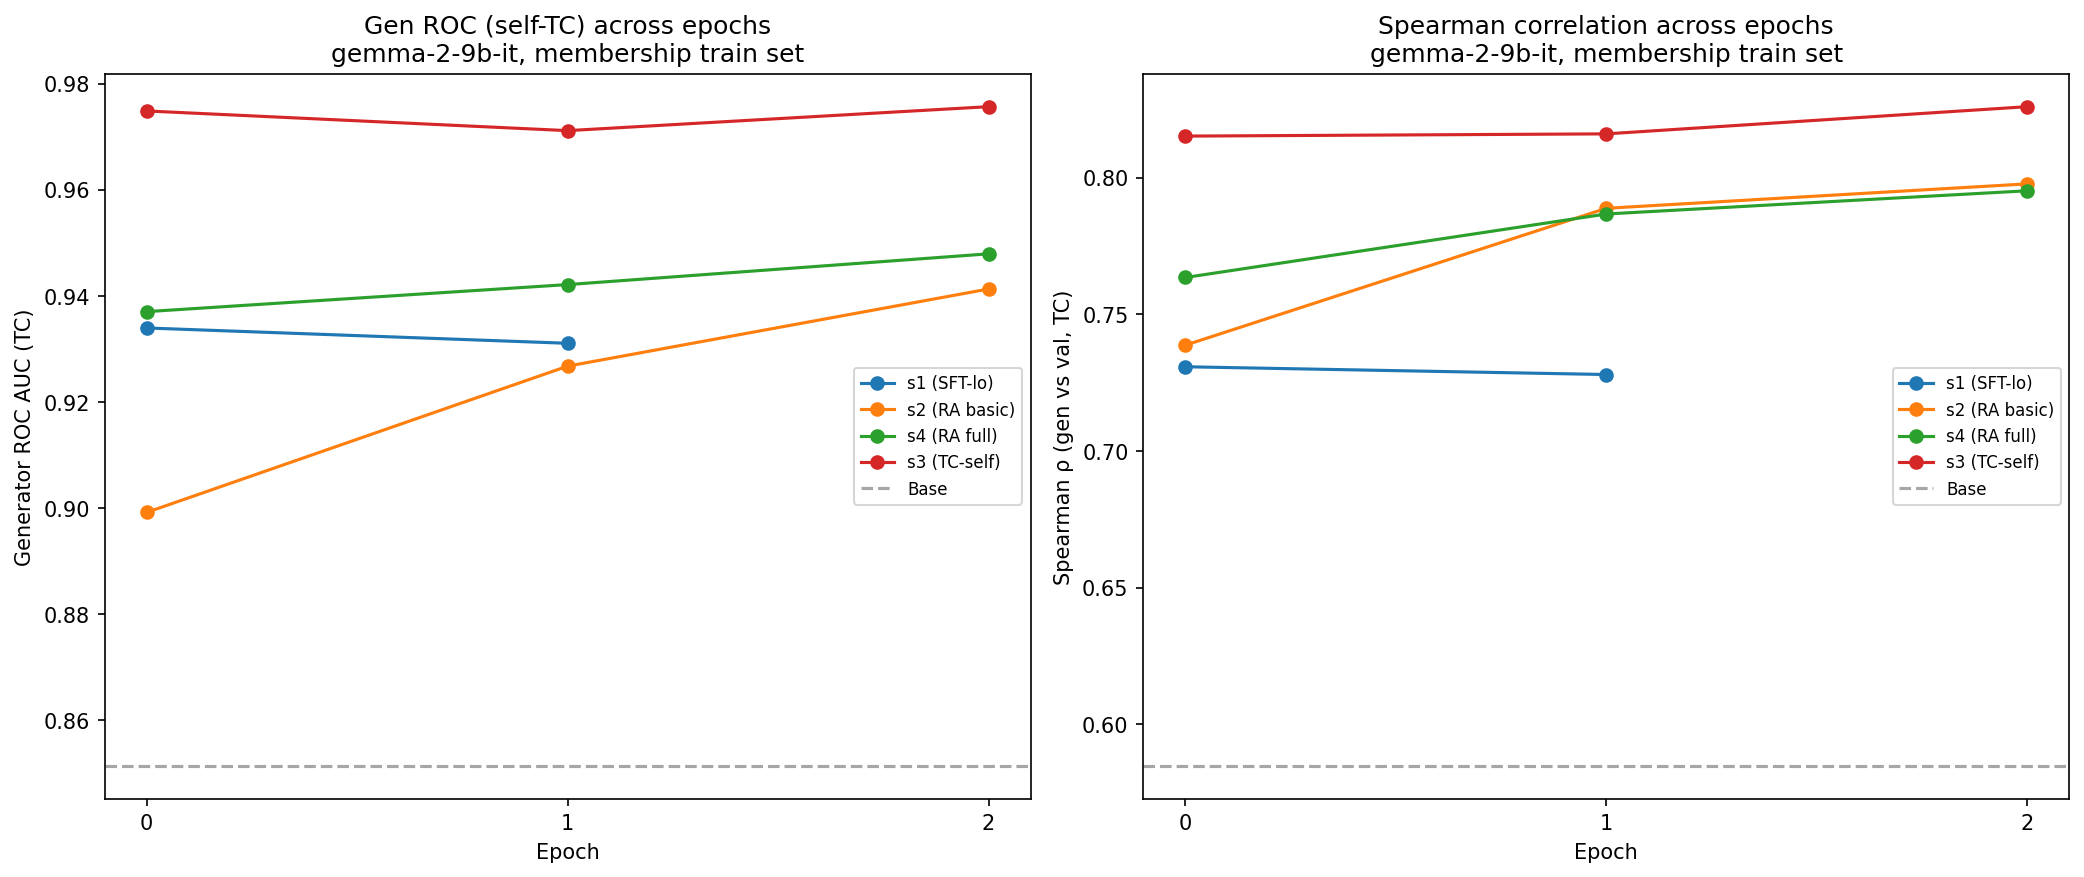
\includegraphics[width=0.95\textwidth]{plots/gemma_membership_dynamics_key_settings.png}
\caption{Training dynamics for gemma membership: Gen ROC and Spearman across epochs.}
\label{fig:dynamics}
\end{figure}

\begin{figure}[H]
\centering
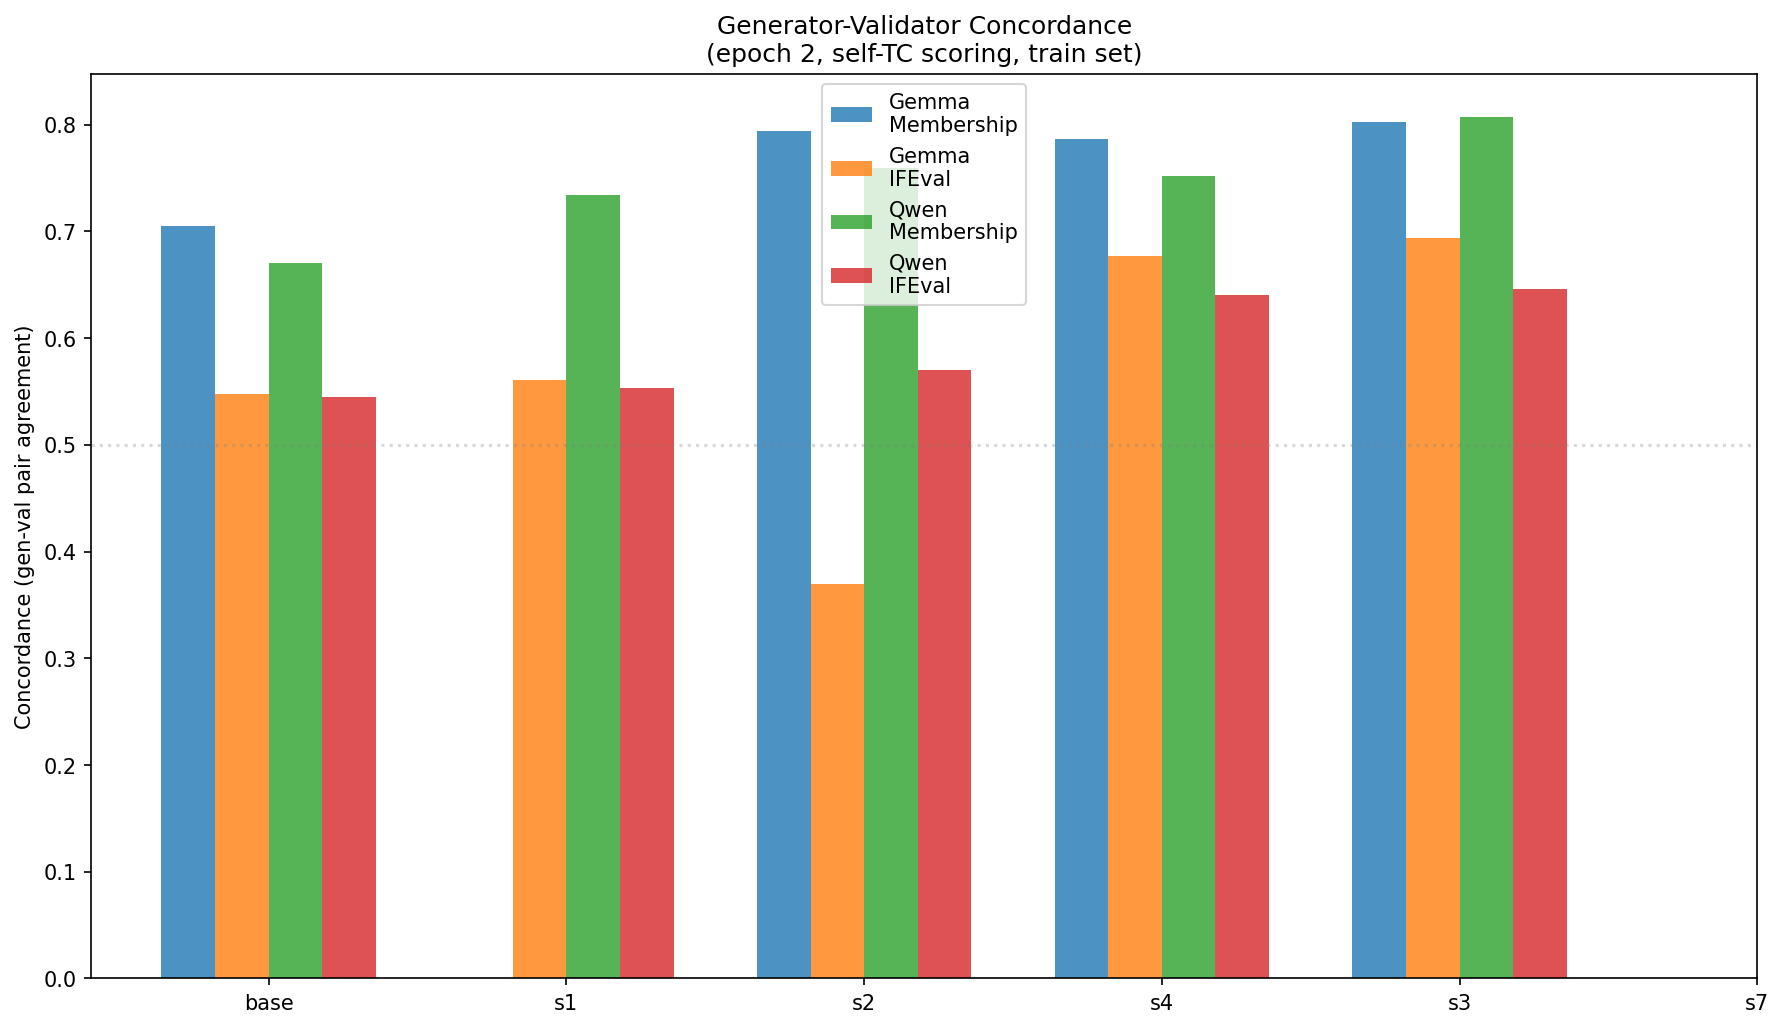
\includegraphics[width=0.95\textwidth]{plots/unified_concordance_comparison.png}
\caption{Concordance across all model/task combinations.}
\label{fig:concordance}
\end{figure}

%% ============================================================
\section{Focused TC Comparison}
%% ============================================================

\subsection{Self-TC vs No-TC (s3 vs s4)}

When evaluated with self-TC scoring, the typicality-corrected models consistently outperform the non-TC baseline (s4):

\begin{itemize}
\item s3 (TC-self, full): $+0.028$ over s4
\item s6 (TC-self fsx, low $\delta$): $+0.023$ over s4
\item s11 (TC-self vlo, no fsx/ppd): $+0.022$ over s4
\item s5 (TC-self basic): $+0.010$ over s4
\end{itemize}

\subsection{Neg-TC vs No-TC (s7 vs s4)}

When evaluated with neg-TC scoring, the improvement from TC-neg training is even larger:

\begin{itemize}
\item s12 (TC-neg vlo): $+0.075$ over s4
\item s7 (TC-neg, full): $+0.072$ over s4
\end{itemize}

This suggests that TC-trained models learn better internal representations that are specifically captured by the matching TC scoring method.

\begin{figure}[H]
\centering
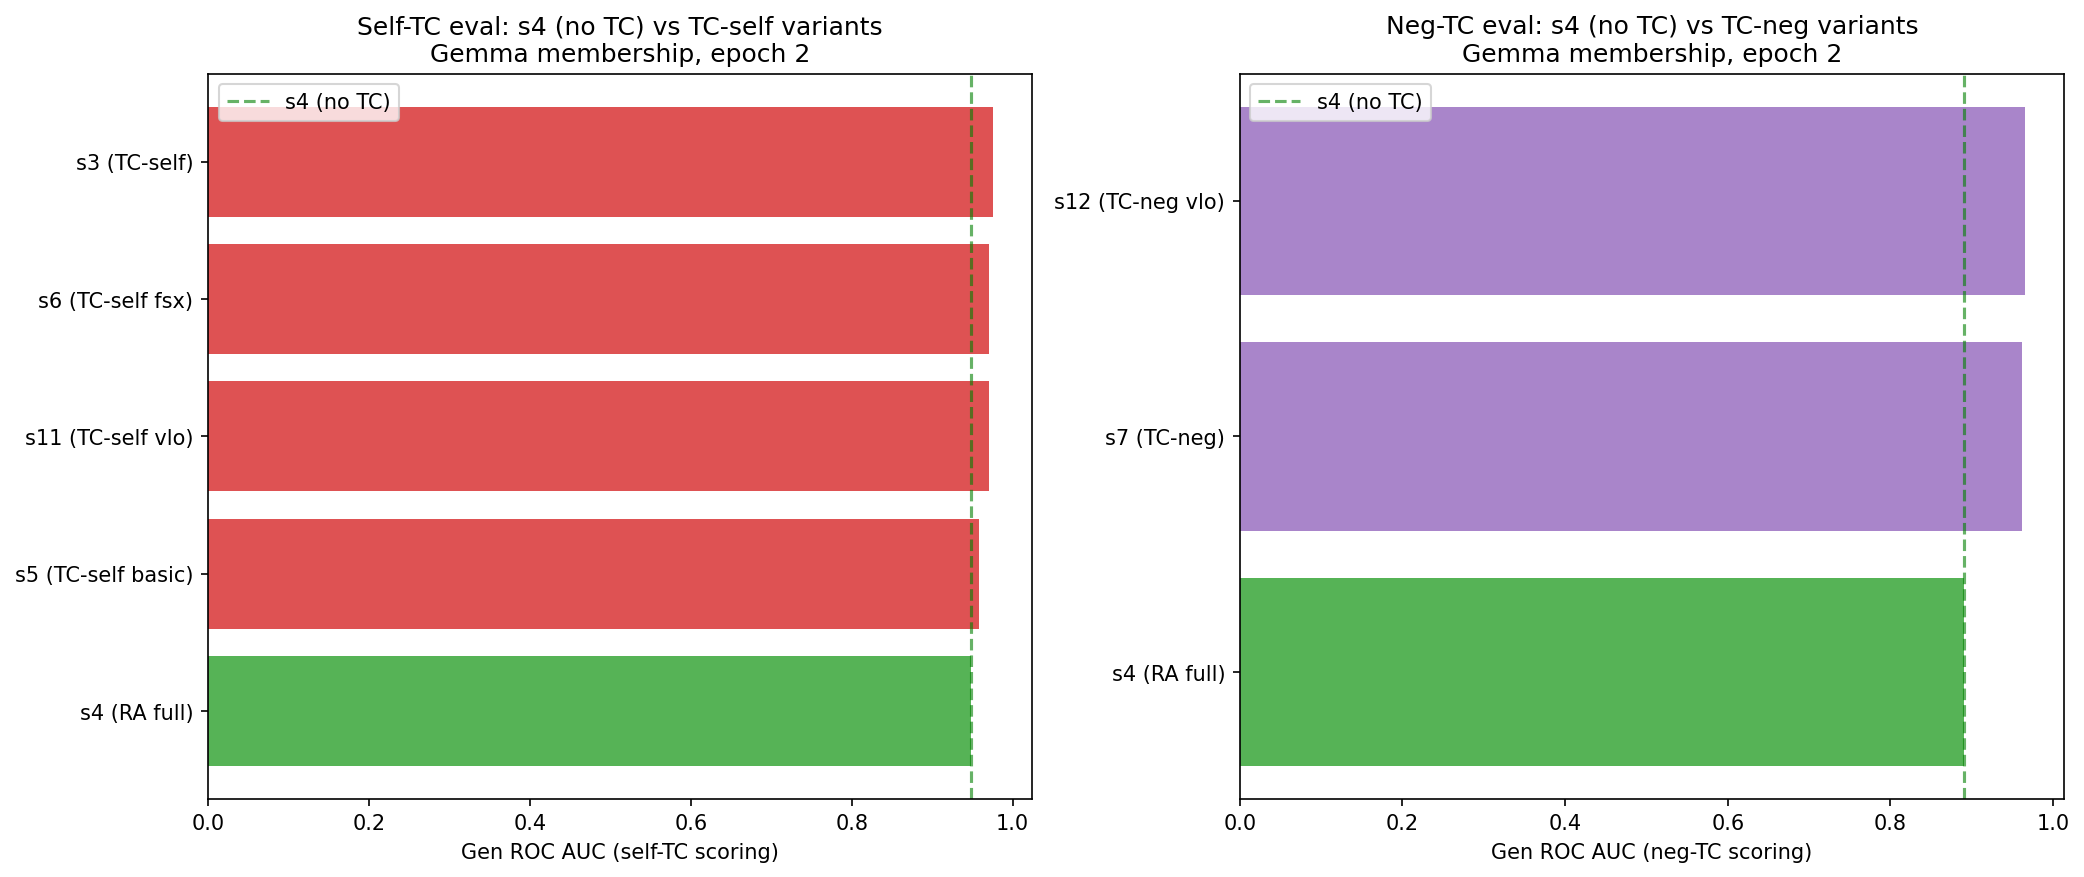
\includegraphics[width=0.95\textwidth]{plots/tc_comparison_self_vs_neg.png}
\caption{TC comparison: self-TC variants (left) and neg-TC variants (right) against s4 baseline.}
\label{fig:tc_comparison}
\end{figure}

\begin{figure}[H]
\centering
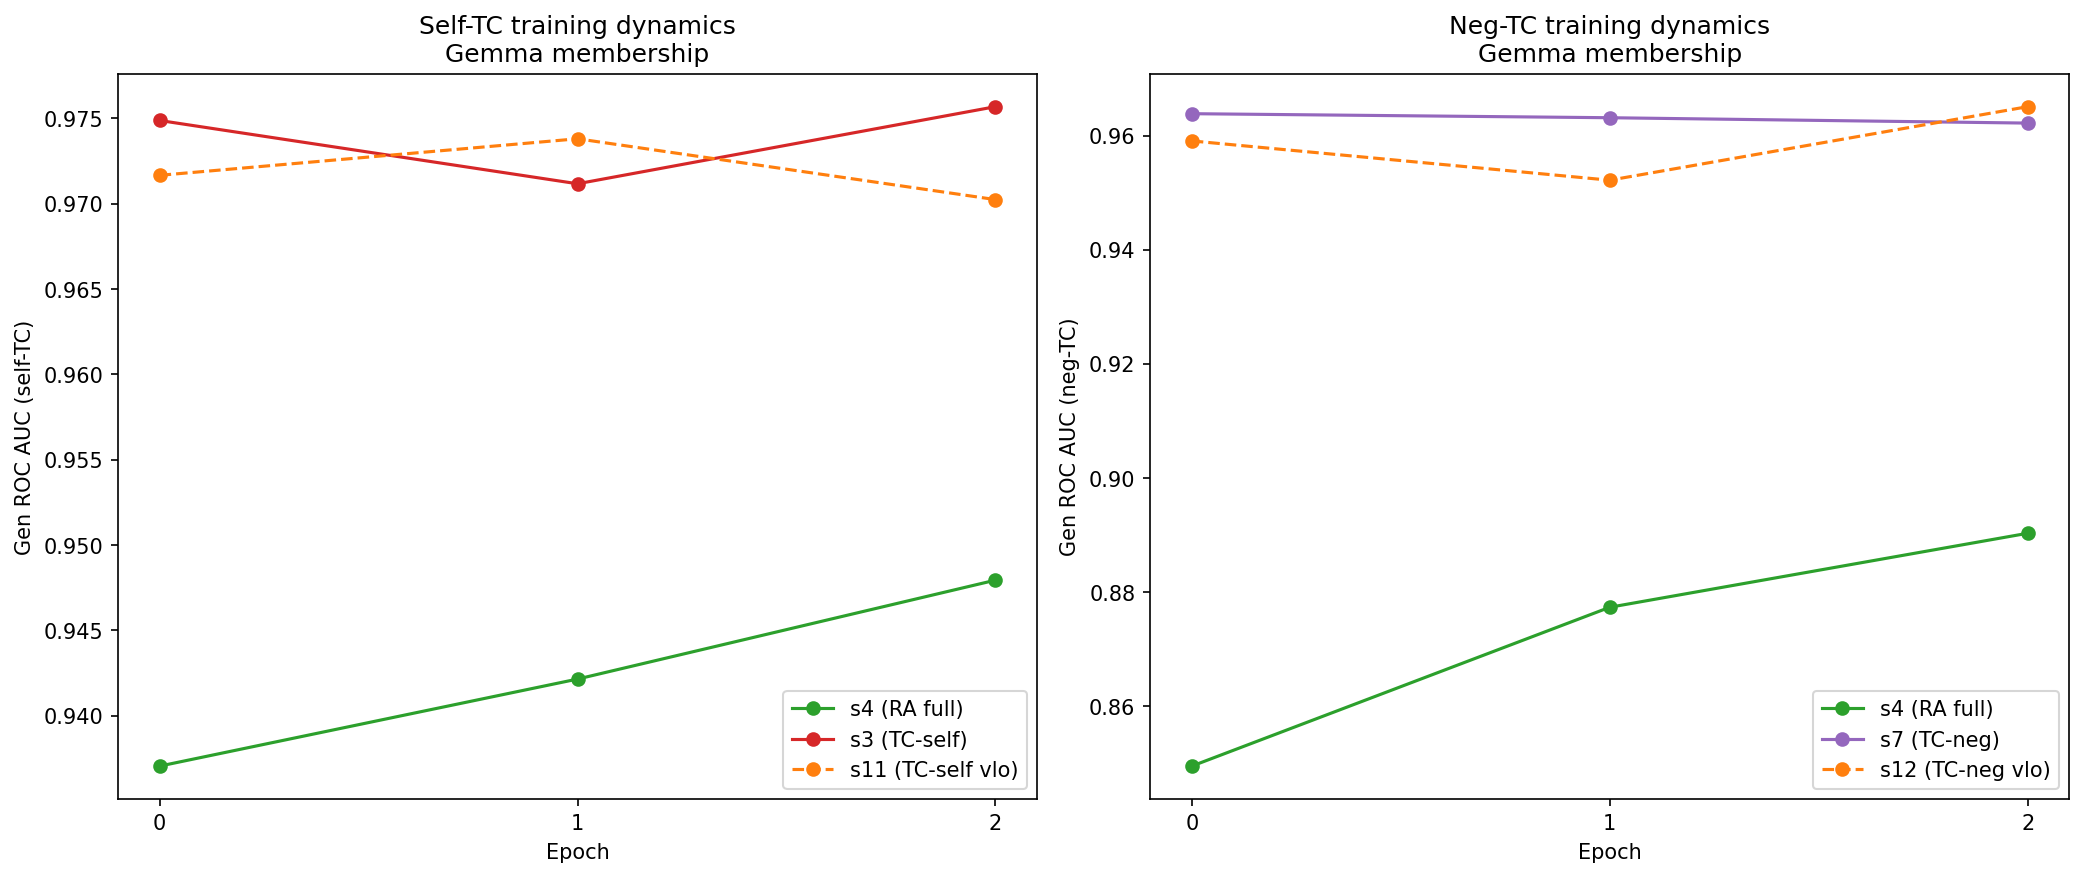
\includegraphics[width=0.95\textwidth]{plots/tc_dynamics_self_and_neg.png}
\caption{Epoch-by-epoch dynamics for TC comparison. TC-trained models converge quickly and maintain advantage throughout training.}
\label{fig:tc_dynamics}
\end{figure}

%% ============================================================
\section{Conclusions}
%% ============================================================

\begin{enumerate}
\item \textbf{RankAlign works when the full method (s4) is used} --- the NLL-V/G constraints are essential for preventing score explosion, especially on complex tasks like IFEval.
\item \textbf{TC-self training (s3) consistently provides the best results} across all metrics (gen ROC, spearman, concordance) and all model/task combinations.
\item \textbf{Basic RankAlign (s2) is unreliable for complex tasks} --- it can actually \emph{hurt} performance (IFEval). The full method is needed.
\item \textbf{Score spread (gen\_delta\_mean) is a powerful training diagnostic} --- values $>$1000 indicate instability. TC-self produces the tightest distributions.
\item \textbf{Concordance is a complementary metric to ROC AUC} --- it directly measures the alignment between generator and validator ranking functions.
\end{enumerate}

\end{document}
